\documentclass[11pt]{article}

\usepackage{ACL2023}

\usepackage{times}
\usepackage{latexsym}
\usepackage[T1]{fontenc}
\usepackage[utf8]{inputenc}
\usepackage{microtype}
\usepackage{inconsolata}

\usepackage{listings}
\usepackage[nolist]{acronym}
\usepackage{placeins}
\usepackage{xcolor}
\usepackage{amsmath}
\usepackage{amssymb}
\usepackage{amsfonts}
\usepackage{etoolbox}
\usepackage{csquotes}
\usepackage{setspace}
\usepackage{graphicx}
\usepackage{booktabs}
\usepackage{multirow}
\usepackage{tablefootnote}
\usepackage{subcaption}


\makeatletter
\def\endthebibliography{%
  \def\@noitemerr{\@latex@warning{Empty `thebibliography' environment}}%
  \endlist
}
\makeatother

\widowpenalty=10000
\clubpenalty=10000
\parfillskip 0pt plus 0.75\textwidth
\makeatletter
\patchcmd{\@sect}{\begingroup}{\begingroup\parfillskip=0pt plus 1fil\relax}{}{}
\patchcmd{\@ssect}{\begingroup}{\begingroup\parfillskip=0pt plus 1fil\relax}{}{}
\makeatother


\title{Project LIT -- Debiasing \acs{NLI} models}

\author{André Trump \And
  Erik Imgrund \And
  Niklas Loeser }

\colorlet{punct}{red!60!black}
\definecolor{background}{HTML}{EEEEEE}
\definecolor{delim}{RGB}{20,105,176}
\colorlet{numb}{magenta!60!black}

\lstdefinelanguage{json}{
    basicstyle=\normalfont\ttfamily,
    numbersep=8pt,
    showstringspaces=false,
    breaklines=true,
    literate=
     *{0}{{{\color{numb}0}}}{1}
      {1}{{{\color{numb}1}}}{1}
      {2}{{{\color{numb}2}}}{1}
      {3}{{{\color{numb}3}}}{1}
      {4}{{{\color{numb}4}}}{1}
      {5}{{{\color{numb}5}}}{1}
      {6}{{{\color{numb}6}}}{1}
      {7}{{{\color{numb}7}}}{1}
      {8}{{{\color{numb}8}}}{1}
      {9}{{{\color{numb}9}}}{1}
      {:}{{{\color{punct}{:}}}}{1}
      {,}{{{\color{punct}{,}}}}{1}
      {\{}{{{\color{delim}{\{}}}}{1}
      {\}}{{{\color{delim}{\}}}}}{1}
      {[}{{{\color{delim}{[}}}}{1}
      {]}{{{\color{delim}{]}}}}{1},
}

\begin{document}

\begin{acronym}
    \acro{CCG}{combinatory categorial grammar}
    \acro{e-SNLI}{Natural Language Inference with Natural Language Explanations}
    \acro{LIME}{Local Interpretable Model-Agnostic Explanations}
    \acro{LM}{Language Model}
    \acro{MCC}{Matthews correlation coefficient}
    \acro{MLM}{Masked Language Model}
    \acro{MultiNLI}{Multi-Genre Natural Language Inference}
    \acro{NLI}{Natural Language Inference}
    \acro{PLM}{Pretrained Language Model}
    \acro{RoBERTa}{Robustly Optimized {BERT} Pretraining Approach}
    \acro{SICK}{Sentences Involving Compositional Knowldedge}
    \acro{SNLI}{Stanford Natural Language Inference}
\end{acronym}

\maketitle
\begin{abstract}
Natural Language Inference (NLI) is the task of deciding on the entailment relation between a hypothesis and a premise. This task is very important for natural language understanding, as it can be used as a building block in more complex tasks. 

We find that the source of predictive performance for \acs{NLI} is found in the fine-tuning procedure. By analyzing the performance and plausibility of the predictions of a fine-tuned model, we conclude that the model is biased for specific phenomena. Furthermore, by evaluating a hypothesis-only model on the training dataset, we show that the training data contains biases that have different strengths when split across different linguistic phenomena.

We try multiple methods for mitigating data bias during training, succeeding in improving predictive performance and reducing bias in the explanations of the model. Furthermore, we recast data from the domain of question answering to the task of \acs{NLI} and apply linguistic techniques to find and generate new examples containing quantifier entailment. By training on the additional training data, the predictive performance is further increased on an easy evaluation set, but reduced on a hard evaluation set, indicating increased bias. We conclude, by confirming most of our hypotheses and showing our learnings.
\end{abstract}

\section{Introduction}


\ac{NLI} is the task of deciding the truthiness of a hypothesis, given a premise. If the hypothesis is true, it can be said to be entailed by the premise. If it is false, it is contradictory to the premise. Otherwise, the truthiness of the hypothesis cannot be determined. For each case, respectively one of the three classes \texttt{entailment}, \texttt{contradiction} or \texttt{neutral} is chosen.

\subsection{Motivation}
The ultimate goal of research in natural language semantics is to represent the meaning of language and how conclusions can be drawn from that. From this point of view, the task of deciding if a sentence in natural language can be entailed by another sentence in natural language is useful and methods to perform such a task could be used as building blocks for many other natural language processing tasks. It has been shown, that a model pre-trained on \ac{NLI} can be used as an effective zero-shot text classifier \cite{yin-etal-2019-benchmarking}.

For \ac{NLI}, complex reasoning is needed in many cases, as minute differences can change the label from \texttt{entailment} to \texttt{neutral} or vice-versa. Furthermore, it has been shown multiple times, that current approaches to \ac{NLI} have many biases in models and datasets and can be easily fooled \cite{hyponly,gururangan-etal-2018-annotation,glockner-etal-2018-breaking}.

Considering the importance of \ac{NLI} for natural language understanding and the current limitations, we set out to improve the state of the art.
\subsection{Research Goals}
As \ac{NLI} is an important task to verify the reasoning capability of \acp{LM}, we want to further analyze it. To this end, we want to show limitations in the current approach to \ac{NLI} and then investigate mitigations to obtain better models.

Thus, our goal is to identify linguistic biases in \acp{LM} for \ac{NLI}, then mitigate those biases by removing biased data in the training procedure and recasting data from other domains to combat the specific biases.
\vspace{1em}

\noindent
We pose the following hypotheses: \vspace*{-0.5em}
\begin{description}
  \setlength\itemsep{-0.3em}
  \item[H1] \acp{PLM} do not contain enough inherent information without fine-tuning for \ac{NLI}.
  \item[H2] Fine-tuned models are biased for some linguistic phenomena.
  \item[H3] The chosen training data is biased and the found bias is not distributed uniformly over linguistic phenomena.
  \item[H4] Mitigating biased data during training results in models with greater predictive performance and less bias.
  \item[H5] Using additional data during training for a specific biased linguistic phenomenon results in models with greater predictive performance and less bias.
\end{description}

\subsection{Structure of our report}
In the rest of this report, we describe our methods in \autoref{sec:method} and thoroughly describe the used models and datasets in \autoref{sec:models_datasets}. We present our experimental setup in \autoref{sec:experiments} and analyze the results in \autoref{sec:results}. Lastly, we formulate our findings regarding the posed hypotheses in \autoref{sec:conclusion}.
\section{Method} \label{sec:method}
\subsection{Probing for \acs{NLI}}
To test the inherent classification performance of \acp{PLM} on \acs{NLI}, a zero-shot baseline is tested. As the \ac{PLM} we plan to use (see \autoref{sec:models_datasets} for further information) is a \ac{MLM}, a mask prediction task is used for zero-shot testing. The template used for that task is \texttt{<premise> <mask> <hypothesis>}, where \texttt{<premise>} is the entire premise sentence with the full stop removed, \texttt{<hypothesis>} is the hypothesis sentence with the first word not capitalized and \texttt{<mask>} is the token that will be predicted.

\begin{table}[ht]
    \centering
    \caption{The discourse markers that were chosen a priori for the zero-shot task with their associated labels.}
    \small
    \begin{tabular}{l | l | l}
        \multicolumn{1}{c|}{Entailment} & \multicolumn{1}{c|}{Neutral} & \multicolumn{1}{c}{Contradiction} \\
        \hline
        as & and  & but \\
        because & also & although \\
        so & or & still
    \end{tabular}
    \label{tab:discourse:markers}
\end{table}

This task is inspired by the discourse prediction task introduced by \cite{dissent}, where a word to relate two sentences to each other is to be predicted. In the same way, we constrain the number of words that are relevant for this task to a short list of typical discourse markers shown in \autoref{tab:discourse:markers} and only compare predictions between those. Each discourse marker is associated with a class. The predicted class is then obtained by taking the class of the discourse marker with maximum probability. As the chosen model tokenizes the start of words with an additional \texttt{Ġ}, we add that to all words but do not show it in the table. We ensured that all words are exactly one single token so that simple masked language modeling can be used.

\begin{table}[ht]
    \centering
    \caption{The words chosen by tuning for the zero-shot task with their associated labels.}
    \small
    \begin{tabular}{l | l | l}
        \multicolumn{1}{c|}{Entailment} & \multicolumn{1}{c|}{Neutral} & \multicolumn{1}{c}{Contradiction} \\
        \hline
        Also & Apparently & Yet \\
        Yes & Perhaps & However \\
        More & Clearly & but \\
        Certainly & Obviously & Unfortunately \\
        yes & Presumably & Otherwise \\
        by &  & Except \\
        Specifically &  & no \\
        Indeed &  & Nearly \\
        Yeah &  & Currently \\
        &  & Sadly \\
        &  & Instead \\
        &  & Not \\
        &  & Previously \\
        &  & Until \\
    \end{tabular}
    \label{tab:discourse:markers:tuned}
\end{table}

Moreover, to test possible improvements by choosing other words, two additional methods are tested. First, we test the simplest possible baseline of just the words \enquote{yes} for \texttt{entailment}, \enquote{maybe} for \texttt{neutral} and \enquote{no} for \texttt{contradiction}. This method does not result in grammatical discourses or sentences, but should still provide a viable baseline, as all words result in similarly ungrammatical sentences, but their embeddings differ. The last method is based on tuning the probing, based on a subset of the training set, that is not used during testing. We tune by obtaining, for each label separately, a count of how many times each token occurs in the top three tokens to be predicted with the chosen template. Then we subtract, for each label and each token, the count of the token for the other labels to filter common words. Lastly, we take all sensible words that have a final count of 15 or more, which are shown in \autoref{tab:discourse:markers:tuned}. This way we account for possibly worse performance that is caused by our choice of discourse markers and choose a potentially better set.

\subsection{Fine-tuning for \acs{NLI}}

Fine-tuning for \acs{NLI} is performed by supervised training on a corpus containing premises, hypotheses and the expected labels. To predict on a single sample, both the premise and hypothesis are fed into the network separated by a separator token. The prediction is then computed by a classification head based on the pooled representation of the complete input. Classification is performed by predicting a vector with three dimensions where each dimension corresponds to one of the labels. The predicted label is the index of the maximum value in that vector. Thus the model is fine-tuned by training it to predict the correct label on the training dataset using the cross-entropy between the predicted class vector and the real class vector as the loss function.

\subsection{Detecting biased data}

By changing the fine-tuning process to only using the hypothesis as input of the model, biases in the data can be found. Such a hypothesis-only model can only correctly predict the labels either by chance or by abusing biases in the data -- it is never correct for the right reasons. It has been shown that for datasets currently used for fine-tuning for \acs{NLI}, hypothesis-only models can be trained that are better than a majority baseline \citep{hyponly}. Thus, it can be concluded that biases in the data must exist that facilitate correct predictions based only on the hypothesis.

We use this fact to find biased samples in the training datasets. A hypothesis-only model can correctly classify samples based on random chance. This does not indicate bias and must be mitigated. We fine-tune three hypothesis-only models on the dataset with different random seeds. Afterward, we declare all samples biased, that are predicted correctly by at least two of the three hypothesis-only models. We also test only declaring samples biased that are predicted correctly by all three hypothesis-only models.

% TODO: Mention how many are deemed biased by at least two and all

\subsection{Mitigating data bias}\label{par:method:mitigating_data_bias}

We employ two methods to remove data bias from the training procedure. The naive method is, to simply remove all samples deemed biased from the training set. By completely removing them from the training procedure, the model cannot be biased by those samples. We call the resulting dataset \texttt{filtered}.

An additional method is introduced by \citet{ensemble}. This method is based on using an ensemble of a frozen biased model and a main model during training and only using the fine-tuned main model during testing. By using the frozen biased model in an ensemble with the main model, the main model can learn to predict based on patterns other than those based on biases. The ensembling can be done by multiplying the prediction of the biased model with the prediction of the main model. The influence of the prediction of the biased model can be reduced by a learned value that is predicted by a secondary head of the main model. By learning to always completely discount the biased model, the model might then learn the biases itself. To prevent this, an additional entropy term is added to the loss function, which punishes the model for discounting the biased prediction too much. As mentioned in the paper, we can also sum the logarithms of the probabilities. We use this, as it should be stabler. \footnote{For more information and justification of this procedure compare with section 3.2 of \cite{ensemble}.}

\subsection{Getting data specific to quantifiers} \label{sec:meth:recasting}

As we will show in TODO, the model is especially biased for samples on quantifiers. To fight this bias, we create additional training data by recasting question-answering-data to the task of \ac{NLI}. The dataset consists of news articles and single sentences that can be entailed when the placeholder is replaced by a particular entity, but cannot be entailed when it is replaced with a different entity. To ensure that the new examples help with the understanding of quantifiers, we only select those containing quantifiers in both the question and the answer. We detect quantifiers by first checking if the word or words the quantifier is consisting of are contained in the sentence. Then, we check if the words have the correct part of speech tags. We do that, as some words we identify as quantifiers can be used in a different sense, such as \enquote{most}, which can be used as an adjective or as a determiner but is not a quantifier when used as an adjective. We use \texttt{nltk} \cite{nltk} for part of speech tagging. The proportion of examples containing quantifiers identified that way is shown in TODO.

From each question-answer pair, we try to create an example with gold labels \texttt{entailment}, \texttt{contradiction} and \texttt{neutral} respectively. The premise for each sample is generated by summarizing the question using a fine-tuned \ac{LM}. If the summary returned contains more than one sentence, then one of those needs to be selected, as the premise should always contain exactly one sentence. We select the sentence by first identifying all named entities in the answer and then selecting the summary sentence with the biggest number of entities contained. If no sentence contains a sufficient amount of answer entities, we do not use this sample.

\begin{table}[ht!]
    \centering
    \caption{Corresponding original and replacement quantifier used for generating contradicting sentences.}
    \small
    \begin{tabular}{l | l}
        \multicolumn{1}{c|}{Original} & \multicolumn{1}{c}{Replacement} \\
        \hline
        a &  no \\
        a few &  many \\
        a large number of &  just a small number of \\
        a little &  a lot \\
        a number of &  zero \\
        a small number of &  a large number of \\
        all &  a few \\
        any &  all \\
        both &  neither \\
        every &  none \\
        each &  just a few \\
        enough &  insufficiently many \\
        few &  many \\
        fewer &  more \\
        less &  more \\
        lots of &  no more than a few \\
        most &  least \\
        many &  few \\
        many of &  few of \\
        much &  limited amount of \\
        neither &  both \\
        no &  most \\
        none of &  several \\
        not many &  each \\
        not much &  much \\
        never &  sometimes \\
        numerous &  limited amount of \\
        plenty of &  shortage of \\
        several &  just one \\
        some &  zero \\
        this &  that \\
        that &  this \\
        the &  none of \\
        whole &  only a part
    \end{tabular}
    \label{tab:contradiction:mapping}
\end{table}

The hypothesis is generated differently for each gold label but all have the same premise. The hypothesis for \texttt{entailment} is simply the correct answer provided by the dataset. The contradicting hypothesis is generated from the answer by replacing the quantifier with an opposing quantifier. We selected the opposing quantifiers based on replacement quantifiers not appearing too often and fitting as an antonym for each quantifier. The mapping from the original quantifier to its replacement can be found in \autoref{tab:contradiction:mapping}.

Lastly, sentences with gold label \texttt{neutral} for the given premise are generated from the answer by using quantifier monotonicity properties similar to the approach chosen by \citet{yanaka-etal-2019-help}. Instead of identifying quantifiers by their semantic tags, we identify them using their part of speech tags, as previously described. Afterward, we also generate a \ac{CCG} derivation using the C\&C Tools \cite{curran-etal-2007-linguistically} and try to extract the nominal and verbal phrases that are part of the quantifier phrase. Next, based on the monotonicity we swap the verbs with either hypernyms or hyponyms found using WordNet \cite{miller-1994-wordnet}. If the quantifier is monotonically rising, we use a hypernym to create a situation, where it cannot be said, if the resulting sentence can be entailed by the original sentence. In the same way, for monotonically falling quantifiers, we use hyponyms to create the samples with \texttt{neutral} as the gold label.

\section{Models and Data Sets} \label{sec:models_datasets}
This section describes the existing models and datasets we use, to perform our experiments and as bases from which we create our models and datasets.

\subsection{Models}
All experiments and variants of the \acs{NLI}-model are based on the pre-trained \acf{RoBERTa} \cite{roberta} in the variation \texttt{roberta-base}, as this provides a good tradeoff of high downstream performance and lower computational requirements. The default pre-trained model is used for the prompt task. All fine-tuned models are based on the pre-trained model with an additional classification head based on the pooled token representation. The classification head is a multilayer perceptron with a single hidden layer of size $768$ and the pooled representation is obtained from the first \texttt{<s>}-token in the output of the \acs{RoBERTa} model. This \texttt{<s>}-token is the equivalent of \acs{RoBERTa} to the \texttt{CLS}-token of other models.

\begin{table}[ht]
    \centering
    \caption{Class distributions for the datasets used}
    \begin{tabular}{l c c c}
        \toprule
        \multicolumn{1}{c}{Gold Label} & \acs{MultiNLI} & \acs{SICK} & \acs{e-SNLI} \\
        \midrule
        Entailment & $137841$ & $2821$ & $190113$ \\
        Neutral & $137152$ & $5595$ & $189218$ \\
        Contradiction & $137356$ & $1424$ & $189702$ \\
        \bottomrule
    \end{tabular}
    \label{tab:datasets:classes}
\end{table}

To create summaries of the articles in the data to be recast, we use a fine-tuned and distilled version of BART \cite{lewis-etal-2020-bart} for text summarization trained on CNN and Daily Mail articles \cite{cnn1,cnn2}. \cite{shleifer2020pretrained} We use a model with all six encoder layers from BART and just six decoder layers named \texttt{distilbart-6-6-cnn}. We use the version trained on CNN/Daily Mail, as this dataset is based on the same data, that we use in our recasting. This implies that the model should work well for the data even when distilled, as there is no shift in domain shift.

\subsection{Datasets} \label{par:models_datasets:datasets}
We use \acs{MultiNLI} \cite{multinli}, \acs{e-SNLI} \cite{esnli} and \acs{SICK} \cite{sick}. In the following, the datasets are described in more detail. Statistics of the datasets can be seen in \autoref{tab:datasets:classes} and \autoref{tab:datasets:sizes}. \autoref{tab:datasets:classes} gives an overview of the distribution of the classes for the datasets and \autoref{tab:datasets:sizes} an overview of the dataset sizes with their respective dataset splits.


\begin{table}[h]
    \centering
    \caption{Dataset split sizes. \acs{MultiNLI} shows the matched/mismatched validation sizes.}
    \begin{tabular}{l  c c c}
        \toprule
        \multicolumn{1}{c}{Split} & \acs{MultiNLI} & \acs{SICK} & \acs{e-SNLI} \\
        \midrule
        Train & $392702$ & $4439$ & $549367$ \\
        Validation & $9815$/$9832$ & $495$ & $9842$ \\
        Test & - & $4906$ & $9824$ \\
        \bottomrule
    \end{tabular}
    \label{tab:datasets:sizes}
\end{table}

\Acf{MultiNLI} \cite{multinli} is a very large corpus that improves upon the \acs{SNLI} corpus by collecting premise-hypothesis pairs from ten different domains. Additionally, only five genres are included in the training dataset and two different validation datasets are provided. One of the validation datasets consists of the same genres as the training dataset while the other validation dataset consists of pairs from five different genres. This allows for cross-domain evaluation and comparisons to in-domain evaluation. Furthermore, including training data from multiple genres is hypothesized to reduce linguistic bias.

\begin{lstlisting}[
    language=json,
    caption={Relevant features of a random data sample from \acs{MultiNLI}.},
    label=code:data:samples:multinli
    ]
{
  "hypothesis": "Product and geography are what...",
  "premise": "Conceptually cream skimming has...",
  "label": 1,
  ...
}
\end{lstlisting}

\autoref{code:data:samples:multinli} shows relevant features of a random sample from the \ac{MultiNLI} dataset. Included are the hypothesis and premise as plain text and the expected label numerically encoded. Additional features such as parses of the premise and hypothesis and the genre of the pair are included in the dataset but irrelevant to this project.

\Acf{SICK} \cite{sick} is a small corpus constructed specifically to address issues with crowd-sourced datasets. It is constructed from two source datasets that describe the same videos or images. The descriptions are first normalized and then expanded to include specific linguistic phenomena. The dataset is much smaller than \acs{SNLI} and \acs{MultiNLI} but is considered to have much higher data quality. The features present in \acs{SICK} are similar to the features present in \acs{MultiNLI}, this is the same numerical label, the premise and the hypothesis as plain text. No parses and genre indications are included, but no further interest is spent on this detail, as those features are not relevant to this project.

\Acf{e-SNLI} \cite{esnli} is a variant of the \acs{SNLI} \cite{snli} corpus that adds up to three natural language explanations and for each explanation an annotation of which words in the premise and hypothesis sentences are deemed important for correct classifications.

\begin{lstlisting}[
    language=json,
    caption={A random data sample from \acs{MultiNLI}.},
    label=code:data:samples:esnli
    ]
{
  "explanation_1": "the person is not neces...",
  "explanation_2": "",
  "explanation_3": "",
  "hypothesis": "A person is training his horse...",
  "label": 1,
  "premise": "A person on a horse jumps over a...",
  "sentence1_highlighted_1": "{}",
  "sentence1_highlighted_2": "",
  "sentence1_highlighted_3": "",
  "sentence2_highlighted_1": "3,4,5",
  "sentence2_highlighted_2": "",
  "sentence2_highlighted_3": ""
}
\end{lstlisting}

\autoref{code:data:samples:multinli} depicts a random sample from the \acs{e-SNLI} corpus including all available features. Comparing it to the features of \acs{MultiNLI} and \acs{SICK}, it is obvious that explanations and highlights of the sentences are added to the data. Up to three different explanations are included and for each explanation, the words in the premise and hypothesis that are relevant to this explanation are provided. The words are provided as indices into the premise and hypotheses starting at zero. For code simplicity, we only use the first explanation.

Additionally, we use a question-answering dataset consisting of CNN/DailyMail articles and corresponding answers that can be entailed by the article \cite{cnn1}. The corpus formulates cloze-style questions by providing the article and a single sentence with a single word replaced by a placeholder. The original task then is to infer what entity would be correct in the place of the placeholder. To pseudonymize the dataset, named entities are replaced with abstract placeholders of the form \enquote{entity\#\#} where \enquote{\#\#} is a positive integer. This is done in the original dataset to test reading comprehension instead of world knowledge.
\begin{lstlisting}[
    language=plain,
    caption={Fomrat of the CNN/Dailymail dataset.},
    label=code:data:samples:cnn-format
]
<URL>

<Article>

<Question>

<Correct Entity>

<Entity Mapping>
\end{lstlisting}

Each sample in the dataset is provided in the format shown in \autoref{code:data:samples:cnn-format} as illustrated by the sample from the CNN dataset in \autoref{code:data:samples:cnn}.

\begin{lstlisting}[
    language=plain,
    caption={A random data sample from the CNN dataset.},
    label=code:data:samples:cnn
]
the job by both @entity25 and @entity26 majority leaders , @entity2 explained . @entity27 leader @entity27 of @entity28 praised @entity9 's smarts and his devotion to the @entity13 . the soft - spoken and bookish...

@placeholder will replace @entity9 , who was parliamentarian for 18 years

@entity8

@entity31:Frumin
@entity2:Reid
@entity1:CNN
@entity0:Washington
@entity13:Senate
@entity27:Mitch McConnell
...
\end{lstlisting}

We replace all placeholders in the article and question with the original entities to provide sensible sentences and such that the model is able to use world knowledge when necessary. Nonetheless, we use the fact that the entities were recognized in the process of recasting the data, as described in \autoref{sec:meth:recasting}

\section{Experiments} \label{sec:experiments}
This section describes all experiments we conduct to evaluate our proposed hypotheses as well as the specific setup we use to perform the experiments including the metrics we use and the splits of our datasets.

\subsection{Testing H1}
\textbf{H1}: \textit{\acp{PLM} do not contain enough inherent information without fine-tuning for \ac{NLI}.}

We test this hypothesis by comparing the predictive performance of a \ac{PLM} and comparing it to the performance of a fine-tuned \ac{LM} for \ac{NLI}. We do that by first evaluating the prompting approach using the pre-trained \ac{RoBERTa} and our three different word groups that map to the different classes, as explained in \autoref{sec:meth:probing}. Additionally, we fine-tune a pre-trained \ac{RoBERTa} model specifically on \ac{NLI} data. 

By comparing the predictive performance of both approaches we can show that fine-tuning is necessary as well as that most of the predictive performance is obtained during fine-tuning. If the hypothesis is confirmed, we would conclude that the fine-tuning procedure should be adjusted instead of the pre-training procedure to obtain better results on \ac{NLI}.

\subsection{Testing H2}
\textbf{H2}: \textit{Fine-tuned models are biased for some linguistic phenomena.}

To test this hypothesis, we evaluate the predictive performance and bias of the model for different subsets of an evaluation dataset. The dataset as well as the metrics for measuring bias are described in \autoref{sec:exp:eval:bias}. Each subset contains only records that represent a particular linguistic phenomenon. This partitioning of the dataset allows for determining which linguistic phenomena the respective model copes better with or worse. If the model performance is significantly better or worse for some linguistic phenomena, we can conclude that differences and biases based on the linguistic phenomena might exist.

The dataset is split into subsets of linguistic phenomena by us using data from WordNet \cite{miller-1994-wordnet}. We consider the linguistic phenomena of synonyms, antonyms, hypernyms, hyponyms, co-hyponyms, quantifiers and numerals. We classify a sample as corresponding to a subset when the phenomenon occurs at least once in words deemed important. We detect synonyms and antonyms by considering, for each important word, all of its synonyms or antonyms respectively and counting occurrences of those in all other words. Hypernyms, hyponyms and co-hyponyms are detected in the same way, where co-hyponyms are words with a common hypernym. Quantifiers are detected in the same way as in our method for recasting data, as described in \autoref{sec:meth:recasting}. Lastly, numerals, that is, numbers and words representing numerical quantities are found by considering the part of speech tags produced by \texttt{nltk} \cite{nltk}.

\subsection{Testing H3}
\textbf{H3}: \textit{The chosen training data is biased and the found bias is not distributed uniformly over linguistic phenomena.}

To test for biases in the training data, we train multiple hypothesis-only models, as described in \autoref{sec:method:detecting_biased_data}. The training data is said to be biased if the hypothesis-only models achieve better performance than could be explained by a majority-only baseline. The bias might manifest in particular words in the hypothesis correlating with specific labels or other structures or phenomena being correlated with a label. This is a data bias, as this is never based on reasoning if the premise can be entailed by the hypothesis, but are always based on statistical correlations only present in this particular data. By comparing the predictive performance of the hypothesis-only model for different linguistic phenomena, as described in the previous section, we can further analyze, for which linguistic phenomena the data is most biased. By analyzing in the described manner, we can learn what linguistic phenomena our mitigation needs to be focussed on.

\subsection{Testing H4} \label{sub:experiments-h4}
\textbf{H4}: \textit{Mitigating biased data during training results in models with greater predictive performance and less bias.}

To test \textbf{H4}, we train three different models and evaluate their predictive performance and bias for different linguistic phenomena. All of the models are based on the methods for mitigating data bias described in \autoref{sec:method:detecting_biased_data}. 

We train two models with filtered datasets. The dataset with all samples removed that are correctly classified by two out of three hypothesis-only models is called \enquote{Filtered 2/3}, the model trained on this dataset is called the same in the following. In the same manner, the dataset and with all samples removed that are correctly classified by all three of the three hypothesis-only models the model trained on it are called \enquote{Filtered 3/3}. As the filtered datasets are smaller and thus, training for the same amount of epochs results in fewer training iterations, we also test the performance of models trained for double the amount of epochs. Those models are called \enquote{Filtered 2/3 longer} and \enquote{Filtered 3/3 longer} in the following.

The third variant we try is based on an ensemble of a frozen biased hypothesis-only model and the fine-tuning model, as previously described. The resulting model is called \enquote{Ensembled}.

\subsection{Testing H5}
\textbf{H5}: \textit{Using additional data during training for a specific linguistic phenomenon the model is biased for results in models with greater predictive performance and less bias.}

To test the effect of additional training data for a specific linguistic phenomenon, we add the recast data obtained using the method described in \autoref{sec:meth:recasting} to the original training dataset. We do not use the filtered dataset from the previous section to test these hypotheses independently of each other. More specifically, we are interested in the performance improvements that can be obtained for that specific linguistic phenomenon, for which we add data and the effects on performance for other linguistic phenomena. To this end, we measure both predictive performance and bias per linguistic phenomenon.

\autoref{tab:new_datasets:classes} gives an overview of the class distributions of our modified datasets, including the filtered datasets from the previous section. \enquote{Recast} is the name of our training dataset with recast data added. Later, the model trained on that dataset will be identified using the name.

\begin{table}[ht]
    \centering
    \caption{Class distributions for the generated datasets}
    \small
    \begin{tabular}{l c c c}
        \toprule
        \multicolumn{1}{c}{Gold Label} &  Filtered 2/3 & Filtered 3/3 & Recast \\
        \midrule
        Entailment & $54147$ & $72939$ & $174531$ \\
        Neutral & $63768$ & $85664$ & $155324$ \\
        Contradiction & $73408$ & $90628$ & $173908$ \\
        \bottomrule
    \end{tabular}
    \label{tab:new_datasets:classes}
\end{table}

\subsection{Evaluation}
To measure the quality of the models, they are tested in two different aspects: The predictive performance and the biases are measured. In the following, we describe our evaluation procedure in more detail.

In general, all models are trained on the train split of \acs{MultiNLI}, unless specified otherwise. All hyperparameters are chosen using short test runs and using the predictive performance on the validation data of \acs{MultiNLI}. The models are trained for three full epochs with a learning rate of $2 \cdot 10^-5$, no weight decay and an effective batch size of $16$.

\paragraph{Predictive Performance}
We define predictive performance as a measure of how often the prediction made by the model is correct. We measure predictive performance based on a dataset of samples, each containing a hypothesis and premise with the gold label known. The gold label is the correct entailment class of the sample.

We use the validation split of \ac{SICK} as our evaluation set during development and the test split of \ac{SICK} for all final results reported here. We use \ac{SICK} for all main testing of predictive performance instead of \ac{e-SNLI} or \ac{MultiNLI}, as it is a harder test set and less biased than both of those. We use the validation split instead of the training split, as we wanted to leave us the option to extend our training dataset by the training split of \ac{SICK}. For tests split by linguistic phenomena, we are using the validation split of \ac{e-SNLI}. As we only want to detect a linguistic phenomenon if it was deemed important for the task, we need a dataset with annotated important words and our only dataset with such annotations is \ac{e-SNLI}.

As the metrics for evaluation, we use the F$_1$-Score and the \ac{MCC} \cite{mcc}. The F$_1$-Score is defined as the harmonic mean of the precision $P$ and recall $R$ for a particular class. So, based on the true positives $\mathrm{TP}$, true negatives $\mathrm{TN}$, false positives $\mathrm{FP}$ and false negatives $\mathrm{FN}$, the F$_1$-Score can be calculated as 

$$\text{F}_1 = 2\cdot \frac{P \cdot R}{P + R} = \frac{2 \cdot \mathrm{TP}}{2\cdot \mathrm{TP} + \mathrm{FP} + \mathrm{FN}}.$$

For multi-class problems such as ours, we compute the macro-average, as this treats each class the same way, independently of their number of samples. The macro-average is computed by first computing the F$_1$-Score for each class and then averaging those. The \ac{MCC} is a measure similar to the Pearson correlation between the prediction and the true label. For the case of two classes, it is defined as 

{\small $$\text{MCC} = \frac{\mathrm
{TP} \cdot \mathrm{TN} - \mathrm{FP} \cdot \mathrm{FN}}{\sqrt{(\mathrm{TP}+\mathrm{FP})(\mathrm{TP}+\mathrm{FN})(\mathrm{TN}+\mathrm{FP})(\mathrm{TN}+\mathrm{FN})}},$$}

and we refer the reader to \citet{mccMultiClass} for the definition of the multi-class variant, as it is not a simple micro- or macro-average but generalized differently. The value range of the \ac{MCC} is $[-1, 1]$, where $-1$ is perfect disagreement, $0$ shows no correlation between prediction and label and $1$ is perfect agreement. Only a perfect classifier can achieve a score of $1$ and any large negative score indicates implementation errors or huge transferability problems between training and test set.

We use the \ac{MCC} and F$_1$-Score, as our evaluation set is heavily imbalanced and biased towards the class \texttt{neutral}, as can be seen in \autoref{tab:datasets:classes}. For imbalanced datasets, metrics such as accuracy might provide a flawed picture of the predictive performance. The macro F$_1$-Score is a popular metric for imbalanced datasets, that we use to alleviate that. Additionally, we use the \ac{MCC}, as it was shown that it is better suited for imbalanced datasets \cite{mccGood}. We use two metrics to provide a more complete picture of the predictive performance than can be summed up into a single number.

\paragraph{Measuring Bias} \label{sec:exp:eval:bias}
To assess the bias of our models, we define bias as making predictions for wrong reasons. As we cannot truthfully know the reasons for a prediction, we use interpretability methods to infer what words might have been important for the prediction. Using the interpretability methods we define bias in the model as assigning importance to words that are not important or not assigning importance to important words. We measure the importance assigned to the words by the model through interpretability methods and control for senseless explanations by also measuring the faithfulness of the explanation.

\ac{e-SNLI} provides natural language explanations for all samples and important words of the hypothesis and premise as annotated by a human annotator. \ac{e-SNLI} provides up to three different explanations for each sample but to simplify our analysis, we select only the first and discard all others. Our analysis is based on the validation split of \ac{e-SNLI}.

We begin the analysis by feeding all samples into our model and calculating the explanations of all explainers provided by ferret \cite{ferret} for each sample individually. Those are Gradients \cite{gradients}, Integrated Gradients \cite{integratedgradients}, \ac{LIME} \cite{lime} and Partition SHAP Values \cite{shap}. We do not limit ourselves to a subset of these explainers as it is not clear which explainer is best suited for all samples and we want to provide a holistic analysis covering every possible angle. 

Afterward, we evaluate the explanations. We differentiate between two aspects of the evaluation of explanations and provides different metrics to measure each of them. The first aspect is Plausibility which assesses how well the explanation aligns with human reasoning. We use the Plausibility to measure the bias of the model which is present by the definition above if the reasoning of the model differs from human reasoning. The metrics provided by ferret for this aspect are token-level \ac{IOU} and F$_1$-Score as well as \ac{AUPRC} calculated between the computed explanation and the human explanation provided by \ac{e-SNLI} \cite{ferret}. 

The second aspect is Faithfulness which is determined by how closely the explanation represents the internal functioning of the model. We use the Faithfulness metrics to determine if the calculated explanations are sensible at all. For this aspect, ferret provides the metrics of Comprehensiveness, Sufficiency and Correlation with Leave-One-Out scores.

Here, too, we do not restrict our analysis to a subset of metrics for the same reasons as above: It is not clear which metric is best suited and we want to get the full picture of metrics as every metric covers a different aspect of the quality of an explanation.

As the last step, we calculate the sum, minimum, maximum, median and mean for every explainer and metric over the whole evaluation dataset. These results allow us to make an informed assessment of which explainer yields the best results and how close the reasoning of the model is to human reasoning.
\section{Results and Analysis} \label{sec:results}
% 1. Accuracy (F1 + MCC) auf SICK und eSNLI einzeln nach Kategorien
% 2. Auf Bias überprüfen: Vergleich vom Modell für wichtig erachtete Token mit von Menschen als wichitg erachtete Tokens
% Visualisierungen:
% - Confusion Matrix (Gentrennt nach Phänomenen)
% - Tabellen Interpretability Metriken (siehe ferret)
In this section the results of our experiments are described and thoroughly analyzed. The results are grouped according to the hypotheses they support.

\subsection{Testing H1}
To test the knowledge contained in \acp{PLM}, we devise prompts that allow for \ac{NLI} predictions, as described in \autoref{sec:meth:probing}. The results obtained using the prompting methods are shown in \autoref{tab:res:prompting}. The word group chosen a priori from the list of discourse markers performs best in F$_1$-Score and second best in \ac{MCC}. The simple word group performs worst in \ac{MCC} but second best in F$_1$-Score. The tuned word group performs best in \ac{MCC} and slightly worse than the simple word group in F$_1$-Score. The difference in F$_1$-Score between a priori and the other word groups is far bigger than the gaps in the \ac{MCC} scores. As the discrepancy is great, we added a metric, the balanced accuracy, to the evaluation that should also be better for imbalanced data than the F$_1$-Score and sometimes more informative than the \ac{MCC} \cite{mccBad}. The balanced accuracy is calculated as the macro-average of the true positive rate of each class \cite{bacc}. Looking at the results in the additional metric, they confirm the ranking obtained by using the \ac{MCC} values. Using this additional fact, we conclude that the \ac{MCC} values are more trustworthy than the F$_1$-Scores for this task.
\begin{table}[ht!]
    \centering
    \caption{Prediction performance when using prompting with different word groups on the \acs{SICK} dataset. The best result is shown in \textbf{bold} and the second-best is \underline{underlined}.}
    \begin{tabular}{l c c c}
        \toprule
        \multicolumn{1}{c}{Word Group} & \acs{MCC} & $\text{F}_1$ & BAcc\\
        \midrule
        A Priori & $\underline{25.51}\%$ & $\mathbf{54.31\%}$ & $\underline{54.11}\%$ \\
        Simple & $20.56\%$ & $\underline{34.40\%}$ & $45.67\%$ \\
        Tuned & $\mathbf{29.11\%}$ & $34.08\%$ & $\mathbf{55.73\%}$\\
        \bottomrule
    \end{tabular}
    \label{tab:res:prompting}
\end{table}

Looking at the resulting \ac{MCC} scores, we can see the expected ordering: The a priori chosen word group is better than the simple words that do not fit into the sentence and the tuned words perform best, as they are tuned on \ac{MultiNLI} to perform better. Interestingly, all approaches, even the simple approach, perform much better than random, which would be an \ac{MCC} of $0$. Nonetheless, compared to the \ac{MCC} score of the fine-tuned model, which is $49.49\%$, the results of using prompting are far worse, even when specifically tuning the prompt words.

\subsection{Testing H2}
\begin{figure}[ht]
    \centering
    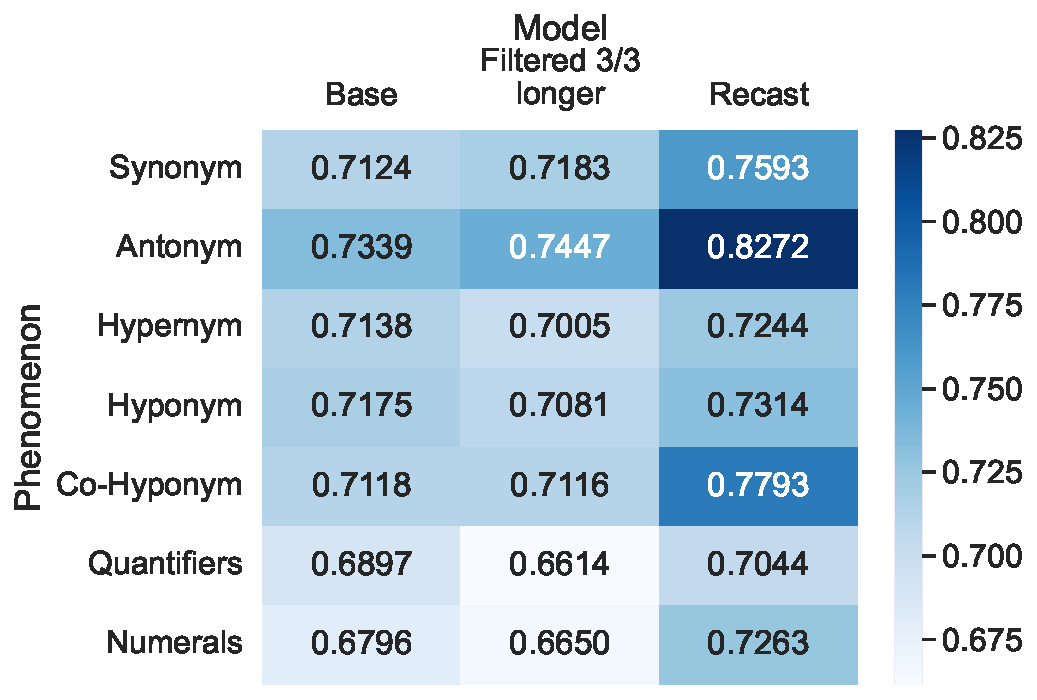
\includegraphics[width=0.9\columnwidth]{./images/metric_heatmaps_phenomena/all_words/base_filtered_recast_matthews_correlation.pdf}
    \caption{\ac{MCC} scores for the models trained on different variants of our training dataset separated by linguistic phenomena.}
    \label{fig:metric-heatmap-phenomena-mcc}
\end{figure}

Figure~\ref{fig:metric-heatmap-phenomena-mcc} depicts the \acs{MCC} scores for our base model separated by linguistic phenomena. Scores for other models are depicted as well but will be described in the following sections. As can be seen in the figure, there are disparities between different phenomena. Antonyms, quantifiers and numerals have the largest disparities of $\geq 0.1$. The base model performs best on the phenomenon of antonyms while performing worst on numerals and quantifiers.

Disparities between phenomena indicate a bias of the model towards certain phenomena. As can be seen in \autoref{fig:metric-heatmap-phenomena-mcc}, the base model performs significantly differently when antonyms, quantifiers or numerals occur.

Analyzing the bias metrics of the model for different linguistic phenomena, we focus on \ac{LIME} as the explanation method of choice. \ac{LIME} has the best faithfulness results across all linguistic phenomena and faithfulness metrics and by a significant margin in many cases. We can see the plausibility metrics obtained using \ac{LIME} in \autoref{tab:res:bias_finetuned}. The complete bias metrics can be found in \autoref{sec:bias_plots_base}, including all explainers and their faithfulness scores.

\begin{table}[ht!]
    \centering
    \caption{Plausibility results obtained using \ac{LIME} as the explainer for different linguistic phenomena of the base fine-tuned model.}
    \begin{tabular}{l c c c}
        \toprule
        \multicolumn{1}{c}{Phenomenon} & \acs{AUPRC} & F$_1$ & \acs{IOU}\\
        \midrule
        Synonyms & $52.58\%$ & $38.50\%$ & $25.57\%$ \\
        Antonyms & $68.08\%$ & $47.68\%$ & $33.23\%$ \\
        Hypernyms & $51.08\%$ & $37.05\%$ & $24.33\%$ \\
        Hyponyms & $50.24\%$ & $36.52\%$ & $23.94\%$ \\
        Co-Hyponyms & $53.56\%$ & $39.86\%$ & $26.57\%$ \\
        Quantifiers & $51.33\%$ & $38.26\%$ & $24.87\%$ \\
        Numerals & $50.22\%$ & $37.55\%$ & $25.02\%$ \\
        \bottomrule
    \end{tabular}
    \label{tab:res:bias_finetuned}
\end{table}

Analyzing the plausibility metrics, they are all in the same range except for antonymy. The results on antonymy are far better than on other phenomena, indicating that the model has a far better understanding of the entailment patterns of antonymy. This is indeed unsurprising, as antonyms often indicate contradictions, which is an easy pattern to learn. More complicated patterns such as the ones by quantifiers and numerals have worse plausibility results. Interestingly, the plausibility is worst for hyponymy. As all of those concepts are interlinked, but classification performance is a lot worse for quantifiers and numerals, the bias is inferred to be the worst for those phenomena. As quantifiers can show complex entailment patterns because of their monotonicity properties, we further focus our analysis on quantifiers.

Figure~\ref{fig:ferret-sample} shows the explanations for the fine-tuned model's classification of a sample from the validation split of the \ac{e-SNLI} dataset obtained using ferret \cite{ferret}. It can be seen that the meaning of the quantifiers in this sample is not considered by the model: The usage of quantifiers in this sample makes it a contradiction but the model attaches high importance only to the quantifier \enquote{all} whereas \enquote{several} has very low importance to the model. The existence of such samples where the model only poorly captures the importance of quantifiers shows that the model is biased after fine-tuning on \ac{MultiNLI}.

\begin{figure*}[t!]
    \centering
    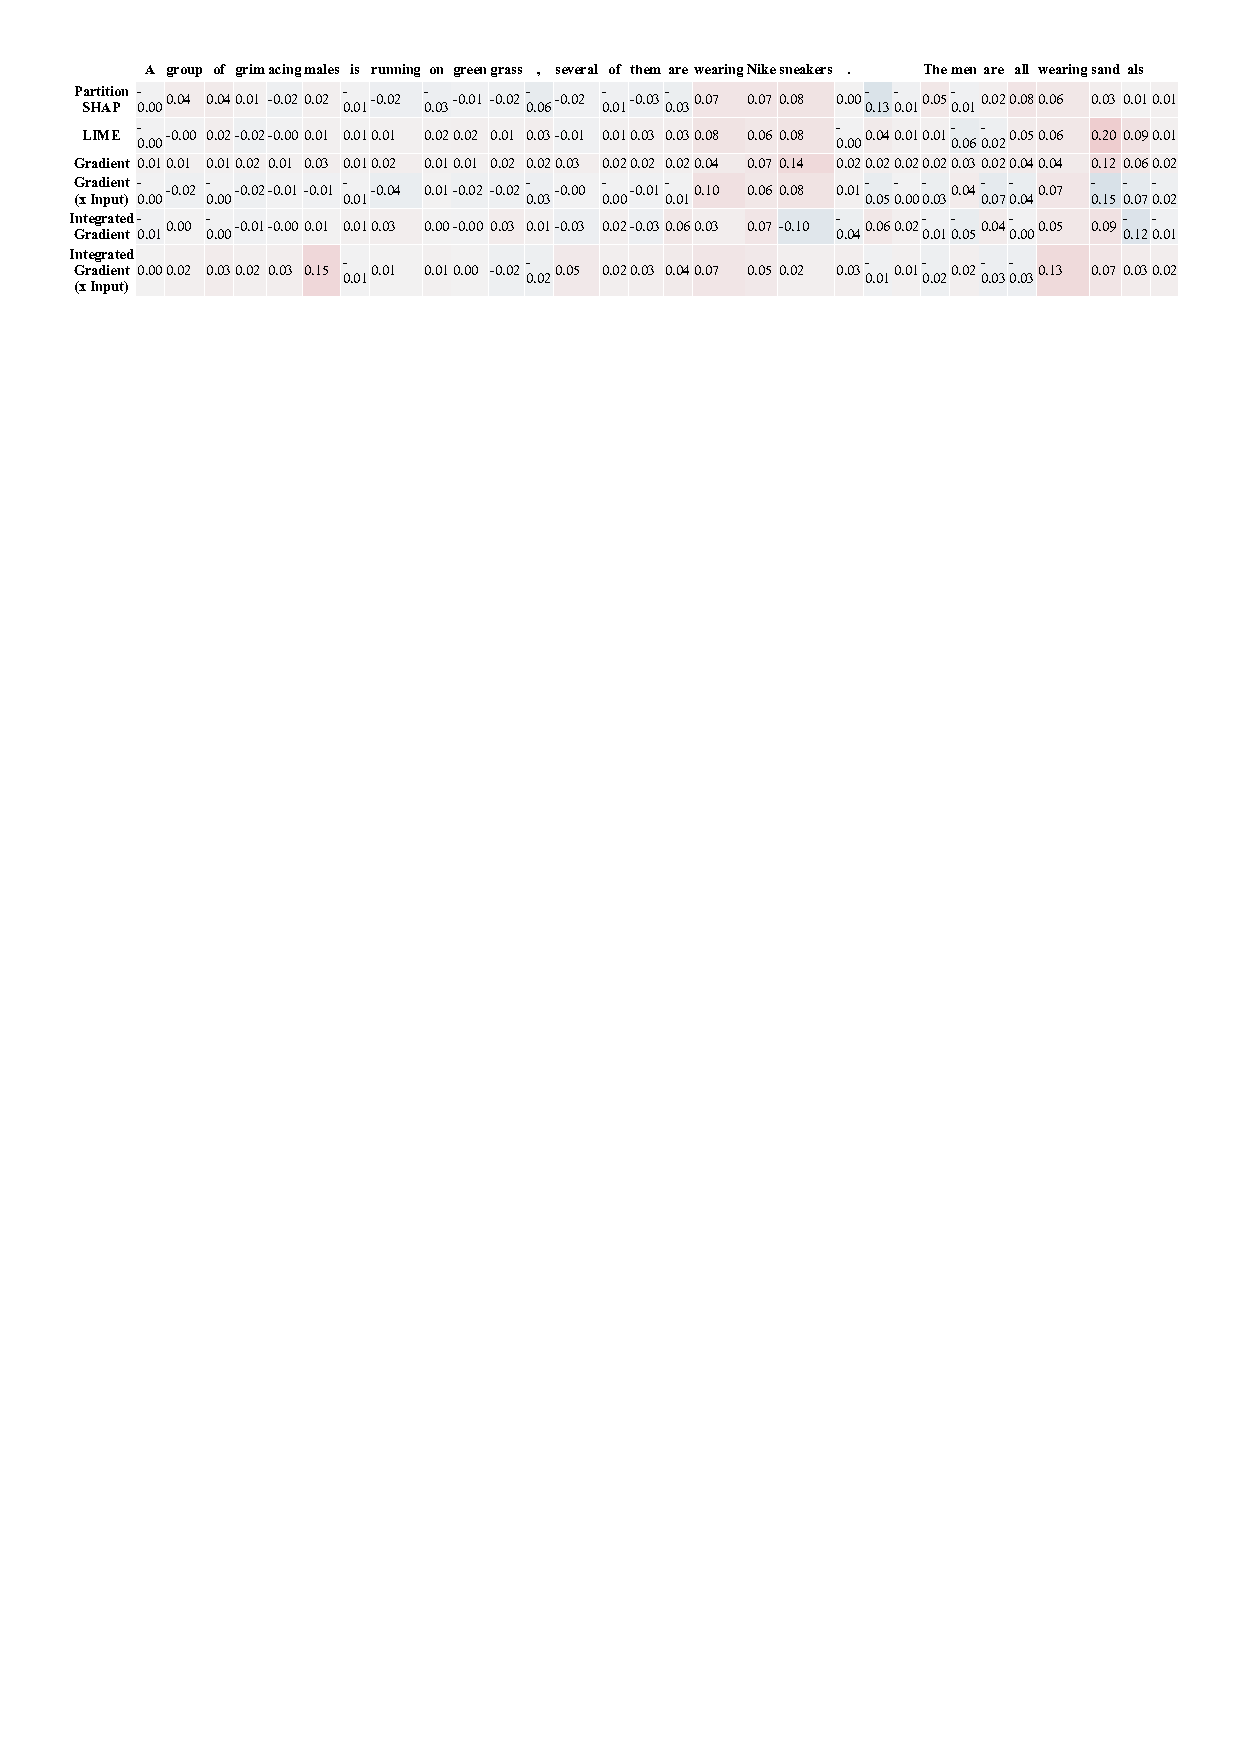
\includegraphics[width=\textwidth]{./images/ferret_sample.pdf}
    \caption{An example of a bad explanation by the base fine-tuned model}
    \label{fig:ferret-sample}
\end{figure*}

\subsection{Testing H3}
Figure~\ref{fig:metric-heatmap-phenomena-mcc-hyponly} depicts the \ac{MCC} scores separated by linguistic phenomena for our model trained on different datasets as described in \autoref{sub:experiments-h4} to show the different predictive performance of the models. The results for the hypothesis-only model were measured on the validation-matched split of \ac{MultiNLI}.

\begin{figure}[ht!]
    \centering
    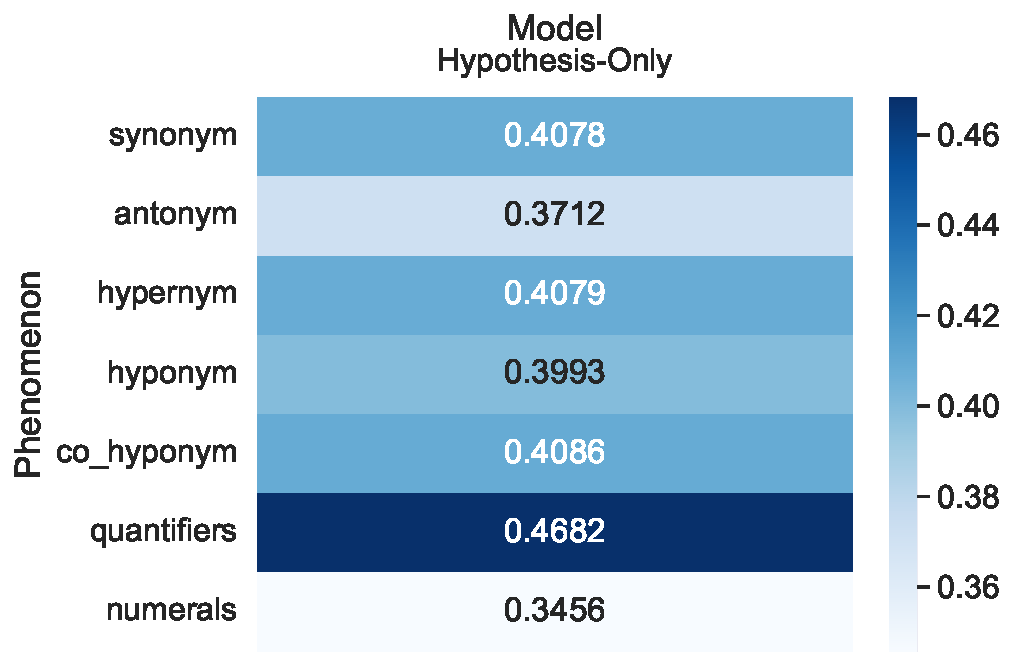
\includegraphics[width=0.9\columnwidth]{./images/metric_heatmaps_phenomena/important_words/hypothesis_only_matthews_correlation.pdf}
    \caption{Matthews Correlation Coefficients for the hypothesis-only model on our training dataset separated by linguistic phenomena}
    \label{fig:metric-heatmap-phenomena-mcc-hyponly}
\end{figure}

In general, the hypothesis-only model shows the expected poor performance: For the phenomena of synonym, hypernym, hyponym and co-hyponym the \ac{MCC} is around $0.4$. The exceptions are antonym, quantifiers and numerals. The model performs particularly poorly on samples that contain antonyms and even worse for numerals. This behavior can be explained by the distribution of phenomena in the dataset shown in \autoref{tab:mnli:phenomena}: Antonyms are found in only $18874$ samples in the training split of \ac{MultiNLI} and numerals only in the hypotheses of $38168$ samples. This makes them the two rarest phenomena in the dataset. 

\begin{table}[ht]
    \centering
    \caption{Phenomenon distribution of the hypothesis of the training split of \ac{MultiNLI}}
    \begin{tabular}{l r}
        \toprule
        \multicolumn{1}{c}{Phenomenon} &  \multicolumn{1}{c}{Number of Samples} \\
        \midrule
        Synonym & $339763$ \\
        Antonym & $18874$ \\
        Hypernym & $117645$ \\
        Hyponym & $124984$ \\
        Co-Hyponym & $381690$ \\
        Quantifier & $48526$ \\
        Numeral & $38168$ \\
        \bottomrule
    \end{tabular}
    \label{tab:mnli:phenomena}
\end{table}

Also comparably rare are samples which contain quantifiers. Nevertheless, the model performs best on samples with an \ac{MCC} of about $0.46$. Since the model cannot possibly determine the meaning of the quantifier for the classification without knowledge of the premise this result is a clear indicator of a bias in the samples that contain quantifiers.

\subsection{Testing H4}
\begin{table}[ht!]
    \centering
    \caption{Prediction performance of our fine-tuned models on the \acs{SICK} dataset. The best result is shown in \textbf{bold} and the second-best is \underline{underlined}.}
    \begin{tabular}{l c c}
        \toprule
        \multicolumn{1}{c}{Model} & \acs{MCC} & $\text{F}_1$ \\
        \midrule
        Base & $49.49\%$ & $56.60\%$ \\
        Hypothesis-Only\tablefootnote{Average of three runs with different seeds} & $14.13\%$ & $40.02\%$ \\
        Filtered $2/3$ & $46.21\%$ & $54.12\%$ \\
        Filtered $2/3$ longer & $36.17\%$ & $52.85\%$ \\
        Filtered $3/3$ & $48.73\%$ & $56.94\%$ \\
        Filtered $3/3$ longer & $\mathbf{52.31\%}$ & $\mathbf{62.04\%}$ \\
        Ensembled & $\underline{51.65\%}$ & $\underline{59.88\%}$ \\
        Recast & $45.33\%$ & $51.64\%$ \\
        \bottomrule
    \end{tabular}
    \label{tab:res:finetuned}
\end{table}

To test this hypothesis, we trained multiple models and evaluated their predictive performance in general and further analyzed the best model. The predictive performance of all models can be seen in \autoref{tab:res:finetuned}, the names follow the names of the datasets introduced in \autoref{sec:experiments}. In this case, a high correlation between the F$_1$-Score and \ac{MCC} can be seen, so we do not need to consult additional metrics. The differences in \ac{MCC} are bigger and the \ac{MCC} was more meaningful when comparing the results of the different prompting methods, therefore we mainly analyze the \ac{MCC} scores.

Unexpectedly, the filtered models perform worse than the base fine-tuned model, even though the data quality should be better. As the models trained on the filtered datasets have been trained for fewer iterations in three epochs, we interpret the inferior results as being because of less training. When evaluating the models trained for more epochs, we can see an improvement for \enquote{Filtered 3/3} and deterioration for \enquote{Filtered 2/3}. This result is only slightly unexpected and can be attributed to \enquote{Filtered 2/3} being more harshly filtered and therefore have even fewer samples which cannot be balanced out by the higher data quality achieved by filtering biased samples more easily. \enquote{Filtered 3/3} shows better performance when trained longer, which indicates it providing a better tradeoff between data quality and data quantity. Therefore, we further analyze \enquote{Filtered 3/3 longer} and use it to compare to the ensembled model.

The ensembled model performs better than the baseline and slightly worse than the filtered model trained longer. This indicates that bias is successfully mitigated during training, as predictive performance on the less biased out-of-domain evaluation set is improved. The performance is still slightly better for the filtered model, we further analyze that instead of the ensemble.

Figure~\ref{fig:metric-heatmap-phenomena-mcc} depicts the \ac{MCC} scores separated by linguistic phenomena for the filtered model compared to the base fine-tuned model. We can see slightly improved performance for antonyms with harshly decreased performance for quantifiers and similar performance for all other phenomena. The decreased performance for quantifiers can be explained by the hypothesis-only model being more accurate on quantifiers and therefore more examples of quantifiers being discarded as biased during filtering. The decreased performance might be explained by either fewer samples of this phenomenon existing after filtering or the evaluation set having the same biases as the training set and thus decreased performance for it that would not exist for a less biased dataset. The increased performance on antonyms but decreased performance on numerals is surprising, as both have poor prediction performance for the hypothesis-only model and thus should not be filtered too much. We interpret that result as random noise or just a general decrease in bias that is randomly effective for antonyms but is not for numerals. Nonetheless, the filtering is beneficial for overall prediction performance, which can be explained by samples not being detected as part of any of our phenomena.

\begin{table}[ht!]
    \centering
    \caption{Plausibility results obtained using \ac{LIME} as the explainer for different linguistic phenomena for the model \enquote{Filtered 3/3 longer}.}
    \begin{tabular}{l c c c}
        \toprule
        \multicolumn{1}{c}{Phenomenon} & \acs{AUPRC} & F$_1$ & \acs{IOU}\\
        \midrule
        Synonyms & $51.77\%$ & $41.87\%$ & $28.43\%$ \\
        Antonyms & $73.32\%$ & $50.12\%$ & $34.81\%$ \\
        Hypernyms & $56.95\%$ & $43.01\%$ & $29.44\%$ \\
        Hyponyms & $55.20\%$ & $42.43\%$ & $28.74\%$ \\
        Co-Hyponyms & $55.14\%$ & $42.43\%$ & $29.04\%$ \\
        Quantifiers & $52.28\%$ & $37.69\%$ & $24.40\%$ \\
        Numerals & $55.24\%$ & $44.01\%$ & $30.18\%$ \\
        \bottomrule
    \end{tabular}
    \label{tab:res:bias_filtered}
\end{table}

Once again, the faithfulness metrics of the explainers are best for \ac{LIME} across all cases, such that we only compare the plausibility results obtained using \ac{LIME}, as seen in \autoref{tab:res:bias_filtered}. The complete results for all explainers and all metrics can be seen in \autoref{sec:bias_plots_filtered}. As we have already found, all plausibility metrics correlate, but we find the biggest differences in \acs{AUPRC} and \acs{IOU}. Looking at the plausibility for different phenomena, we see the same patterns as for the base finetuned models with slight differences. The model performs similarly on all phenomena except for antonyms, for which it is a lot better. Nonetheless, differences show in the weaknesses of the model: Whereas the base fine-tuned model was weak for quantifiers, numerals and hyponyms, the improved model is weak only for quantifiers and synonyms. A notable exception to the correspondence between \acs{AUPRC}, F$_1$ and \acs{IOU} are the results for synonyms, that show a weak \acs{AUPRC} score but strong F$_1$ and \acs{IOU} scores. Because of this, we consider the \acs{IOU} instead of the \acs{AUPRC} in the comparison of the base and filtered model in \autoref{tab:res:bias_comparison}.

\begin{table}[ht!]
    \centering
    \caption{Plausibility \acs{IOU} obtained using \ac{LIME} as the explainer for different linguistic phenomena compared between the base model and \enquote{Filtered 3/3 longer}.}
    \begin{tabular}{l c c}
        \toprule
        \multicolumn{1}{c}{Phenomenon} & Base & Filtered 3/3 longer \\
        \midrule
        Synonyms & $25.57\%$ & $28.43\%$ \\
        Antonyms & $33.23\%$ & $34.81\%$ \\
        Hypernyms & $24.33\%$ & $29.44\%$ \\
        Hyponyms & $23.94\%$ & $28.74\%$ \\
        Co-Hyponyms & $26.57\%$ & $29.04\%$ \\
        Quantifiers & $24.87\%$ & $24.40\%$ \\
        Numerals & $25.02\%$ & $30.18\%$ \\
        \bottomrule
    \end{tabular}
    \label{tab:res:bias_comparison}
\end{table}

Comparing the filtered model to the base model, we can see a clear increase in plausibility across all phenomena except for quantifiers. This indicates, that the bias is successfully mitigated during training and as such the model is less biased. We interpret the result of quantifiers not being improved, in such a way, that simply removing the impact of biased samples of quantifiers is not enough to teach the model quantifier entailment patterns. This result of more bias for quantifiers is analogous to the decreased predictive performance for quantifiers. We can conclude, that the filtering process helps create a stronger model with less bias, but additional measures need to be taken, to improve performance for quantifiers.

\subsection{Testing H5}
To test this hypothesis the predictive performance of the recast model has been tested on both the \ac{SICK} dataset and the \ac{e-SNLI} dataset.

The results obtained on the \ac{SICK} dataset can be seen in \autoref{tab:res:finetuned}. Unexpectedly, the performance of the model on the \ac{SICK} dataset dropped significantly compared to the base finetuned model both in terms of the \ac{MCC} and F$_1$-Score. This can be explained by the fact that both \ac{e-SNLI} and \ac{MultiNLI} are variants of the \ac{SNLI} dataset and are therefore rather similar to each other. In contrast, \ac{SICK} is from a completely different domain and was specifically constructed to reveal issues with crowdsourced datasets such as \ac{e-SNLI} and \ac{MultiNLI}.

Figure~\ref{fig:metric-heatmap-phenomena-mcc} depicts the result of the recast model on the \ac{e-SNLI} dataset per linguistic phenomenon compared to the other models. The model's performance on samples that contain quantifiers and have been determined to be biased has indeed been improved by the addition of the recast data compared to the base finetuned model. We interpret this as a result of decreased bias in the quantifier samples caused by the additional recast data.

Interestingly, also the performance on all other linguistic phenomena has increased, but most drastically on antonyms on which the model's performance increased by almost ten percentage points. Also on all other linguistic phenomena, the model's performance has increased by at least two percentage points. This behavior can be explained by the increased amount of training data also showing examples of other linguistic phenomena.

\section{Conclusion} \label{sec:conclusion}
Following the structure of the previous sections, we conclude our findings for each of the posed hypotheses.

\paragraph{H1:} \textit{\acp{PLM} do not contain enough inherent information without fine-tuning for \ac{NLI}.}

Our results clearly show that using prompting of \acp{PLM} for \ac{NLI} is not sufficient to get good predictive performance. We have tuned the prompt on a training dataset achieving better results and showing that the prompting can be improved. Our prompting results are still far worse than simple fine-tuned models, indicating that the information contained in the \acp{PLM} is not sufficient to complete this complex task, but additional training is needed to learn the correct reasoning patterns. With further tuning of the prompts, better results might be achieved, but our current results indicate that most of the predictive performance for \ac{NLI} is obtained from fine-tuning. This indicates that the fine-tuning procedure should be changed to improve the properties of the resulting model.

\paragraph{H2:} \textit{Fine-tuned models are biased for some linguistic phenomena.}

By comparing the predictive performance across different linguistic phenomena, we show differences in accuracy for certain linguistic phenomena. This correlation between the presence of certain linguistic phenomena and accuracy indicates a bias in the model. Furthermore, we analyze the plausibility of explanations of the model's predictions, showing that the predictions are mostly plausibly explained but with a clear difference between linguistic phenomena. Plausibility is low for classes with low predictive performance, indicating a correlation between predictive performance and bias of the model in some cases. From the evidence gathered, we conclude that the model is indeed biased for numerals and quantifiers.

\paragraph{H3:} \textit{The chosen training data is biased and the found bias is not distributed uniformly over linguistic phenomena.}

By training a hypothesis-only model and showing better performance than could be explained by a majority-only baseline, we clearly show biases in the chosen training data. By analyzing it for different linguistic phenomena, we show that the examples are most biased for quantifiers and focus our efforts on mitigating bias on this phenomenon. 

\paragraph{H4:} \textit{Mitigating biased data during training results in models with greater predictive performance and less bias.}

From the presented results, this hypothesis can be confirmed. We have shown, that either filtering biased samples or mitigating biased samples by use of a special training procedure, both result in greater predictive performance. Furthermore, we have shown, that for the model trained on filtered data, the explanations generated by interpretability methods are more plausible, indicating reduced bias. Nonetheless, it must be noted, that using filtering must be tuned in both the amount of filtering and training length, complicating the training procedure.

\paragraph{H5:} \textit{Using additional data during training for a specific linguistic phenomenon the model is biased for results in models with greater predictive performance and less bias.}

This hypothesis can be confirmed only partially. We have shown that using additional training data can result in greater predictive performance for all linguistic phenomena, even though only data specifically tuned for one phenomenon is added. Nonetheless, performance on the hard evaluation set is greatly decreased by the additional training data. Seeing that predictive performance is increased for \acs{e-SNLI} and decreased for \acs{SICK}, we interpret the model as being more biased. This could be mitigated by applying additional debiasing methods in combination with the additional recast data.

\paragraph{Summary of our Results}

We pose the following learnings from our results:

\begin{enumerate}
    \item \acp{LM} for \ac{NLI} need to be fine-tuned for this task.
    \item \ac{NLI} models get their performance from the fine-tuning procedure, which can be adjusted to modify the final predictive performance and biases of the model.
    \item Higher plausibility of the explanations of the model results in higher predictive performance on out-of-domain datasets.
    \item Current \acp{LM} are biased for quantifiers and numerals, as those phenomena sometimes require complex reasoning.
    \item Training data for \ac{NLI} is biased in multiple ways.
    \item \acs{LIME} is the explainer with the biggest faithfulness for our experiments by a significant margin.
    \item Sometimes, multiple plausibility metrics are needed to get a complete picture.
    \item Mitigating bias during training by filtering biased samples improves final predictive performance and reduces bias in the explanations.
    \item The amount of filtering must be tested and tuned to achieve improvements.
    \item Using additional data can significantly improve performance.
    \item Additional data needs to be of high quality to improve performance for hard datasets such as \acs{SICK}.
\end{enumerate}

\FloatBarrier
\bibliography{lib}
\bibliographystyle{acl_natbib}

\FloatBarrier
\appendix
\section{Bias plots} \label{sec:bias_plots}

The figures \ref{fig:ferret-mnli-synonym}, \ref{fig:ferret-mnli-antonym}, \ref{fig:ferret-mnli-hypernym}, \ref{fig:ferret-mnli-hyponym}, \ref{fig:ferret-mnli-co-hyponym}, \ref{fig:ferret-mnli-quantifiers} and \ref{fig:ferret-mnli-numerals} depict the faithfulness and plausability metrics obtained by ferret. The explainers are listed on the x-axis. \enquote{Ig} is shorthand for the integrated gradient explainer. \enquote{Igmby} is the integrated gradient explainer multiplied by the inputs.

\begin{figure*}[h!]
    \centering
    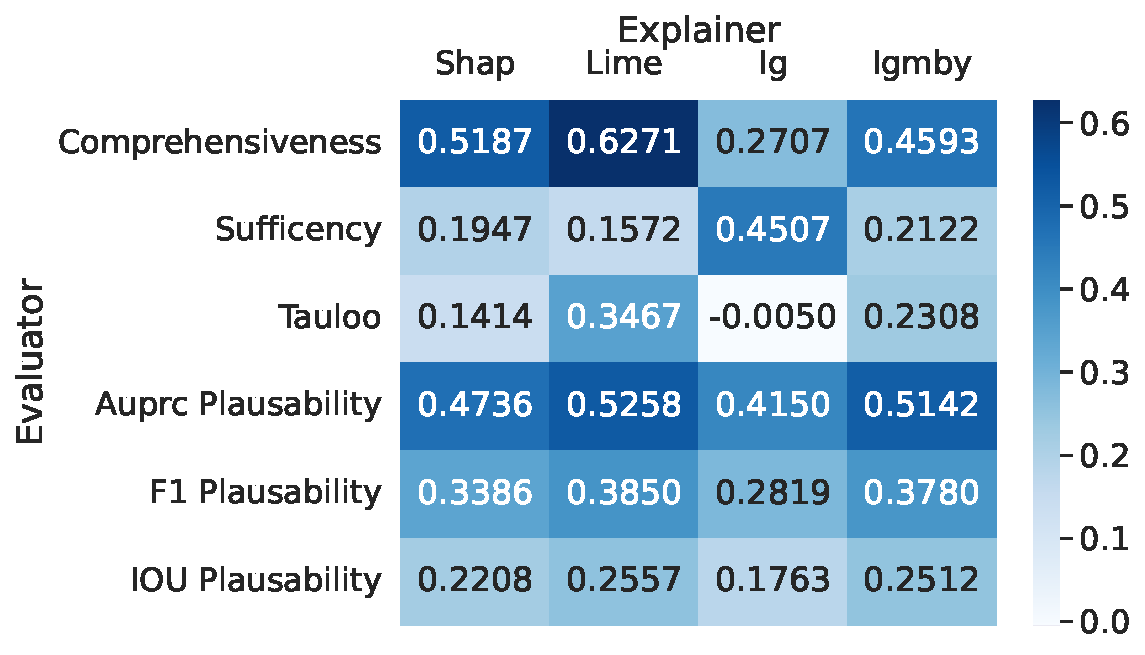
\includegraphics[width=\textwidth]{./images/ferret_heatmaps_phenomena/default_mnli/synonym.pdf}
    \caption{Faithfulness and plausibility of the Base model measured on \acs{e-SNLI} filtered for synonymy}
    \label{fig:ferret-mnli-synonym}
\end{figure*}

\begin{figure*}[h!]
    \centering
    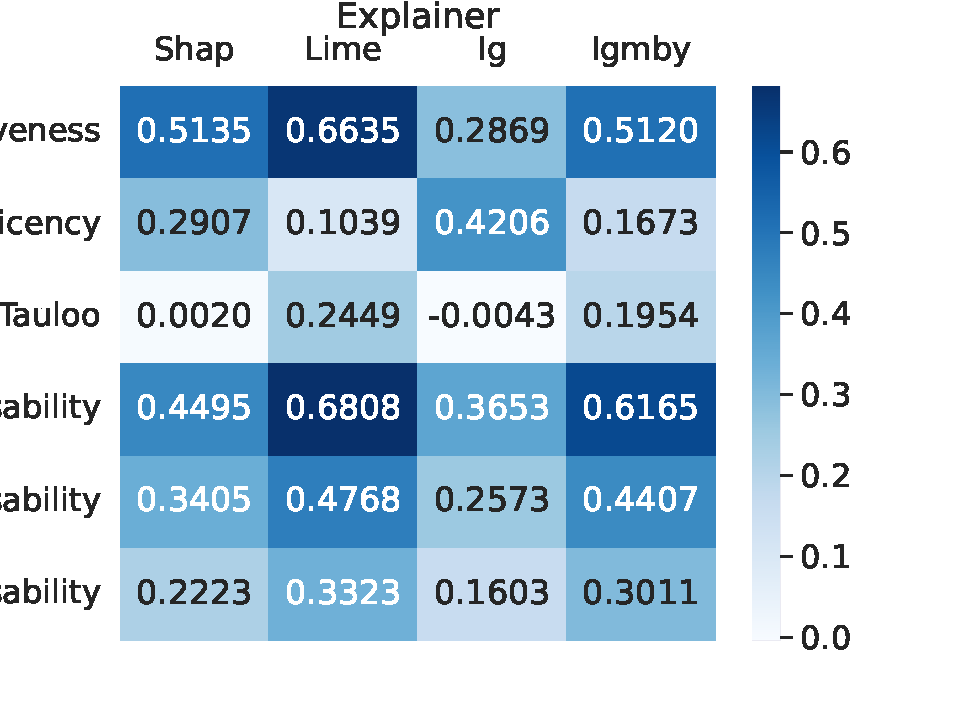
\includegraphics[width=\textwidth]{./images/ferret_heatmaps_phenomena/default_mnli/antonym.pdf}
    \caption{Faithfulness and plausibility of the Base model measured on \acs{e-SNLI} filtered for antonymy}
    \label{fig:ferret-mnli-antonym}
\end{figure*}

\begin{figure*}[h!]
    \centering
    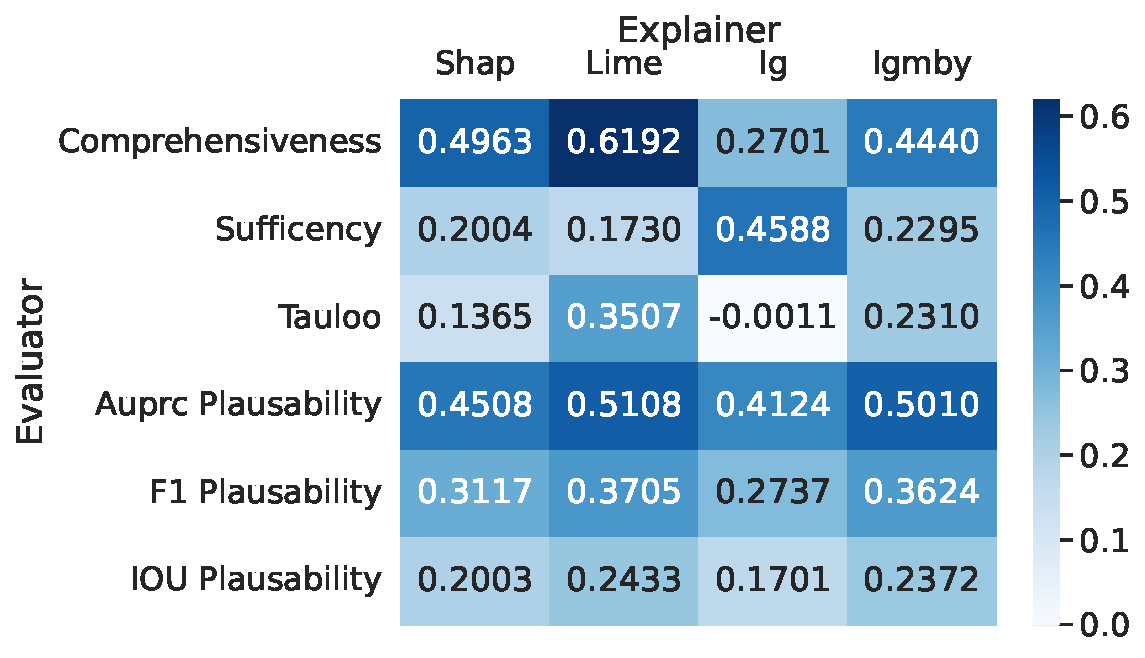
\includegraphics[width=\textwidth]{./images/ferret_heatmaps_phenomena/default_mnli/hypernym.pdf}
    \caption{Faithfulness and plausibility of the Base model measured on \acs{e-SNLI} filtered for hypernymy}
    \label{fig:ferret-mnli-hypernym}
\end{figure*}

\begin{figure*}[h!]
    \centering
    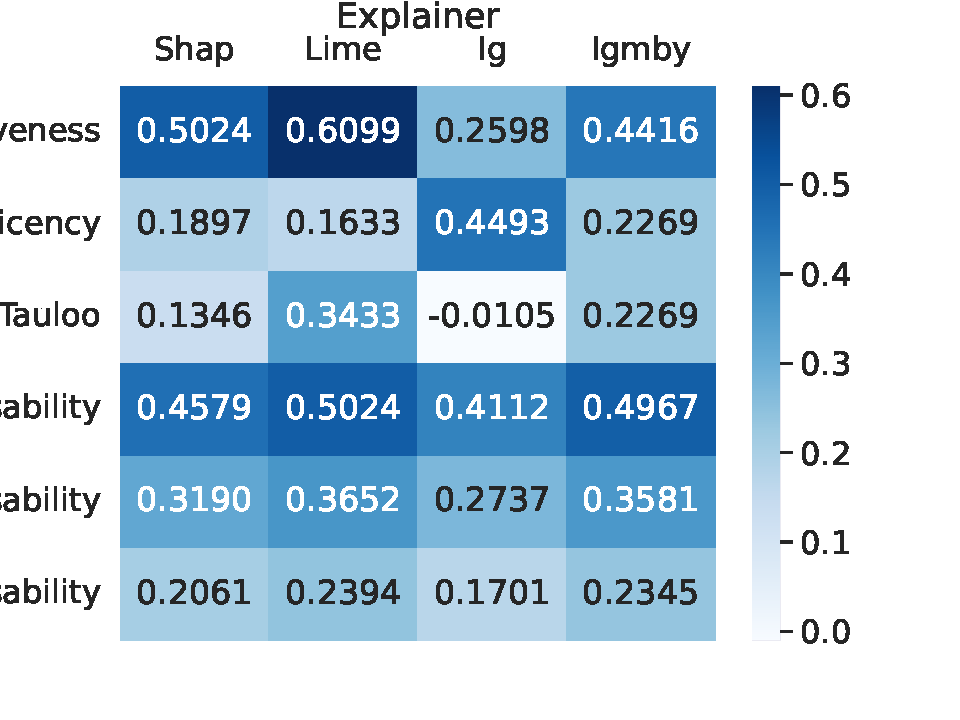
\includegraphics[width=\textwidth]{./images/ferret_heatmaps_phenomena/default_mnli/hyponym.pdf}
    \caption{Faithfulness and plausibility of the Base model measured on \acs{e-SNLI} filtered for hyponymy}
    \label{fig:ferret-mnli-hyponym}
\end{figure*}

\begin{figure*}[h!]
    \centering
    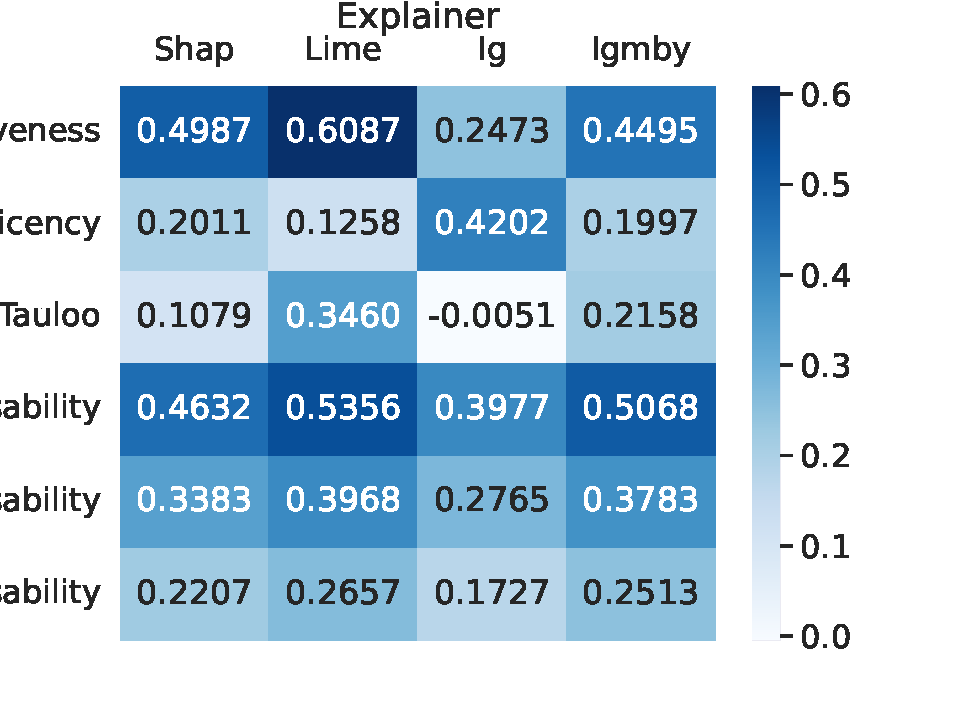
\includegraphics[width=\textwidth]{./images/ferret_heatmaps_phenomena/default_mnli/co_hyponym.pdf}
    \caption{Faithfulness and plausibility of the Base model measured on \acs{e-SNLI} filtered for co-hyponymy}
    \label{fig:ferret-mnli-co-hyponym}
\end{figure*}

\begin{figure*}[h!]
    \centering
    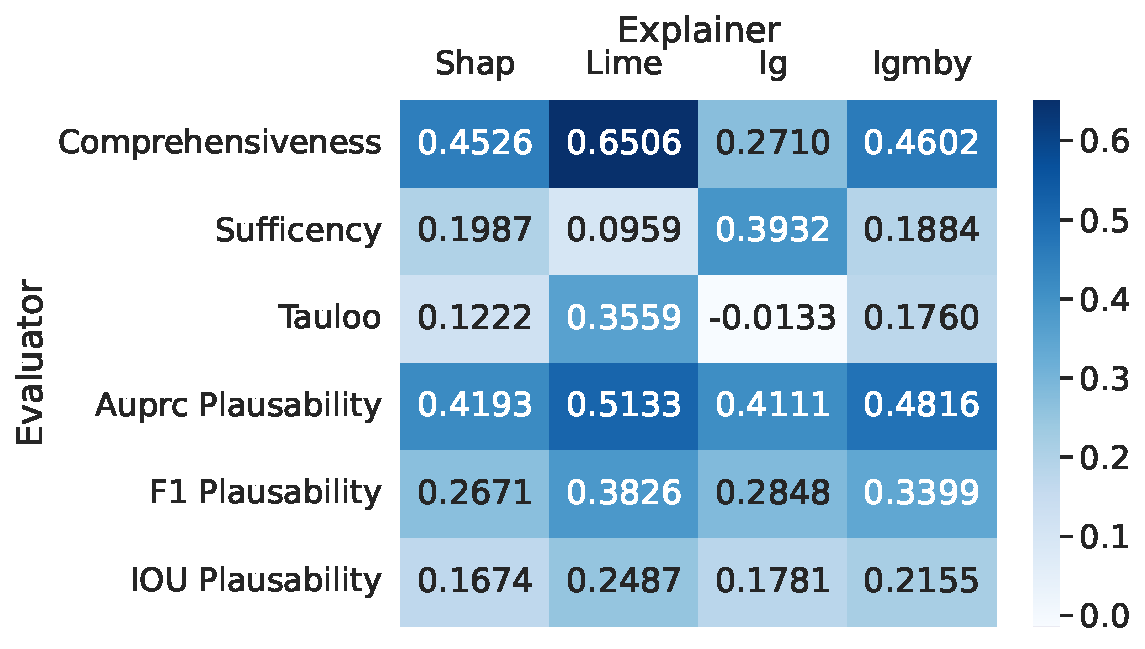
\includegraphics[width=\textwidth]{./images/ferret_heatmaps_phenomena/default_mnli/quantifiers.pdf}
    \caption{Faithfulness and plausibility of the Base model measured on \acs{e-SNLI} filtered for quantifiers}
    \label{fig:ferret-mnli-quantifiers}
\end{figure*}

\begin{figure*}[h!]
    \centering
    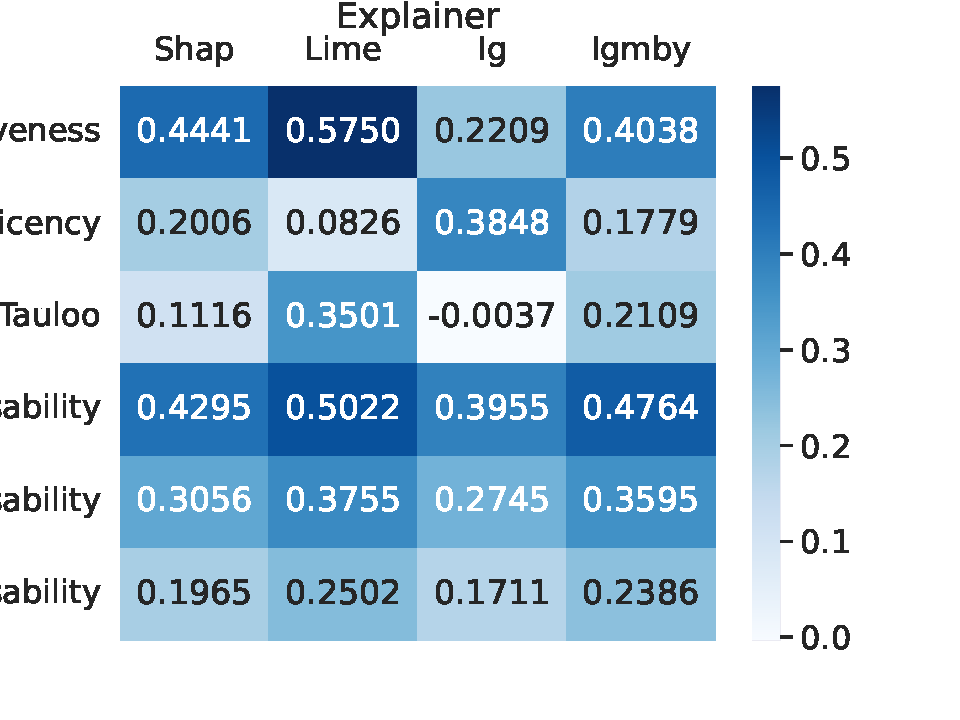
\includegraphics[width=\textwidth]{./images/ferret_heatmaps_phenomena/default_mnli/numericals.pdf}
    \caption{Faithfulness and plausibility of the Base model measured on \acs{e-SNLI} filtered for numerals}
    \label{fig:ferret-mnli-numerals}
\end{figure*}


\end{document}
